\documentclass[a4paper,10pt]{article}
\usepackage[utf8]{inputenc}
\usepackage[T1]{fontenc}
\usepackage[english]{babel}
\usepackage[a4paper]{geometry}
\usepackage{graphicx}
\usepackage{float}


\title{Software Architectures\\ Assignment 5 : Software Visualizations}
\author{Arnaud Rosette, Simon Picard}

\begin{document}
\maketitle
\section{Exercise 1 : Analyzing the web portal application with an existing visualization}
\subsection{Chosen visualization}
As the assignment required, we chose a predefined visualization of Moose. We decided to use the Blueprint complexity visualization because it highlights the complexity of a class, the cohesion inside a class, the coupling between different classes and the class hierarchy. So this visualization is able to show us the application architecture from a close perspective as well as a large perspective.
\begin{figure}[H]
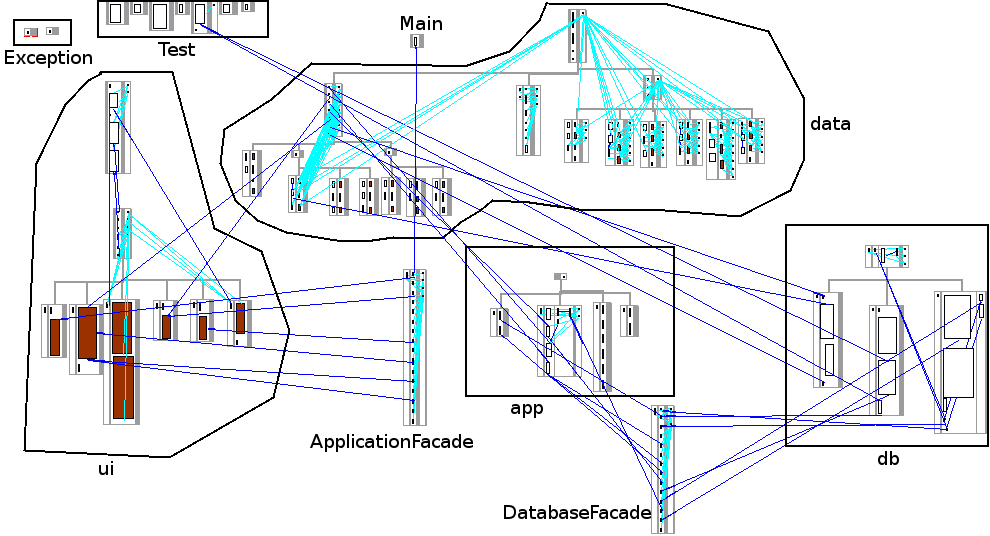
\includegraphics[width=\textwidth]{src/blueprint.png}
\centering
\caption{Class hierarchy Blueprint of the web\_portal application}
\end{figure}
\subsection{Useless classes}

\subsection{3-tier architecture}

\subsection{Cohesion}

\subsection{Coupling}

\section{Exercise 2 : Building your own visualization with Mondrian}
\end{document}
